\chapter{Envelope geometry parameterization}
\label{geometry}

Geometry parameterization is an essential part of the design exploration and shape optimization process and there are several methods of generating parametric geometries. Since our ultimate aim of the project is to study different configurations of the non-body-of-revolution shapes and select the best one satisfying our needs. Thus there is a need to parameterize the geometry. Initial attempts were made using unconventional generalised methods like polynomial fitting, ruled surface between splines, NURBS etc. The idea is to define any shape using design variables of not more than 10 because the complexity (time taken, number of function evaluations and memory consumption) of an optimizing problem increases exponentially[\citenum{OsamaAbdulGhani2013}] with number of design variables. So, it has to be as less as possible provided every combination of them gives a meaningful airship shape.

\section{Modified Gertler parameter technique}

In this study, Gertler Series 58 Shape Generator are used for airship envelope generation. This sub-section explains the formulation of this shape generator in detail. It starts with a six degree polynomial equation in 2-D as stated in Eq. \ref{eq21}.
\begin{equation}
\label{eq21}
z^2 = a_1y + a_2y^2 + a_3y^3 + ... + a_ny^n	
\end{equation}
where $a_1$, $a_2$, $a_3$,..., $a_n$ are the shape coefficients, whose values are driven by  geometrical parameters, viz., $m$ (location of maximum diameter), $r_o$ (Nose radius), $r_1$ (tail radius) and $C_p$ (prismatic coefficient), shown in Fig. \ref{fig:cp}. Here $ V_{env} $ is the volume of the envelope and $ V_{c} $ is volume of enclosing cylinder.
\begin{figure}[H]
	\centering
	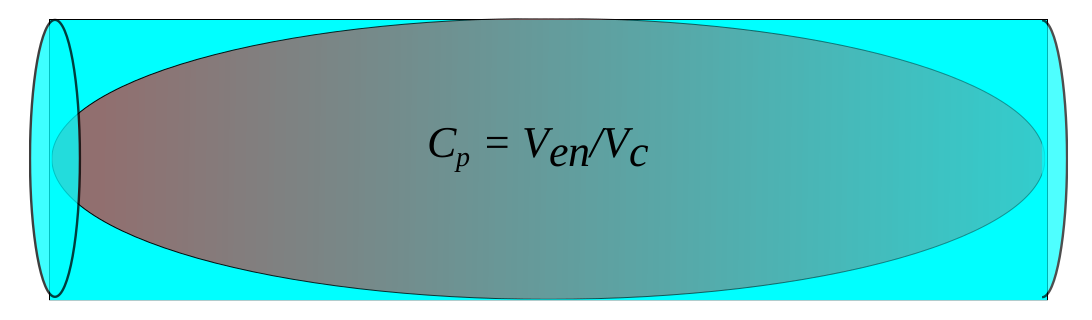
\includegraphics[width=0.7\linewidth]{rnd/c_p_definition.png}
	\caption{Definition of $ Cp $ [\citenum{alam2017thesis}]}
	\label{fig:cp}
\end{figure}
By satisfying the various constraints applicable for the shape of a stratospheric airship envelope, the final equations can be obtained in terms of these shape coefficients. To satisfy the constraints applicable for an airship envelope, we apply the conditions $z = 0$, when $y = 1$; $z = 1/2$, when $y = m$ and $\dfrac{dz}{dy} = 0$, when $y = m$, to obtain:
\begin{equation}
a_1 + a_2 + a_3 + ... + a_n = 0	
\end{equation}
\begin{equation}
a_1m + a_2m^2 + a_3m^3 + ... + a_nm^n = \frac{1}{4}	
\end{equation}
\begin{equation}
a_1 + 2a_2m + 3a_3m^2 + ... + na_nm^{n-1} =0	
\end{equation}
Radius of curvature $R$ for any curve can be given as:
\begin{equation}
R = \pm \dfrac{1}{\dfrac{d^2Y}{dZ^2}}\left[1+\left(\dfrac{dY}{dZ}\right)^2\right]^{3/2}
\label{RoC}	
\end{equation}
Eq. \ref {RoC} can be expressed in a  dimensionless form as:
\begin{equation}
\label{eq24}
r = \pm \dfrac{1}{\dfrac{d^2y}{dz^2}}\left[1+\frac{L^2}{D^2}\left(\dfrac{dy}{dz}\right)^2\right]^{3/2}	
\end{equation}
Differentiating Eq. \ref{eq21} successively with respect to y we get:
\begin{equation}
\label{eq22}
2z = \left(a_1 + 2a_2y +...+ na_n^{n-1}\right)\dfrac{dy}{dz}
\end{equation}
and
\begin{equation}
\label{eq23}
2 = \left(a_1 + 2a_2y +...+ na_n^{n-1}\right)\dfrac{d^2y}{dz^2} + \left[2a_2 + ...+n(n-1)a_n^{n-2}\right]\left(\dfrac{dy}{dz}\right)^2
\end{equation}
In Eq. \ref{eq22}, if $a_1\ne 0$ then it can be said that when $x = 0$, $\dfrac{dy}{dz} = 0$, and hence from the Eq. \ref{eq23}, that
$\dfrac{d^2y}{dz^2} = \dfrac{2}{a_1}$. Consequently substituting these values in Eq. \ref{eq24} we can get:
\begin{equation}
\label{eq25}
a_1 = 2r_o
\end{equation}
where $r_o$ is the radius of curvature at the nose. If, on the other hand $a_1 = 0$, then $r_o = 0$, i.e., the body has pointed nose, which is not possible for an inflated envelope. Hence, Eq. \ref{eq25} is valid for both the cases.\\
Similarly, when $y = 1$, $z = 0$ and from Eq. \ref{eq22},     $\dfrac{dy}{dz} = 0$, unless:
\begin{equation}
\label{eq26}
a_1 + 2a_2 + 3a_3 +...+na_n = 0
\end{equation}
Hence, Eq. \ref{eq24} and Eq. \ref{eq23} give:
\begin{equation}
\label{eq27}
a_1 + 2a_2 + 3a_3 +...+na_n = -2r_1
\end{equation}
where $r_1$ is the radius of curvature at the tail. Different signs are taken in equation of $r_o$ and $r_1$ because of the nature of slope at the points $y = 0$ and $y = 1$ respectively.

Volume of the envelope ($ V_{env}) $ can be expressed as:
\begin{equation}
V_{env} = \int_{0}^{l}\pi Z^2 dY = \pi d^2L\int_{0}^{1}z^2dy	
\end{equation}
substituting for $z^2$ from Eq. \ref{eq21} we get,
\begin{equation}
\dfrac{1}{2}a_1	+ \dfrac{1}{3}a_2 + \dfrac{1}{4}a_3+ ... + \dfrac{1}{n+1}a_n = \dfrac{1}{4}C_p
\end{equation}

The aforementioned six constraints can be expressed in the form of a six degree polynomial as follows:
\begin{equation}
z^2(0) = 0
\end{equation}
\begin{equation}
z^2(1) \implies a_1 + 2a_2 + 3a_3 +...+na_n = 0
\end{equation}
\begin{equation}
\dfrac{dz}{dy}\Big|_0 \implies a_1= 2r_o
\end{equation}
\begin{equation}
\dfrac{dz}{dy}\Big|_1 \implies a_1 + 2a_2 + 2a_3 +...+na_n = -2r_1
\end{equation}
\begin{equation}
z^2(m)\implies a_1m + a_2m^2 + a_3m^3 + ... + a_nm^n = \frac{1}{4}	
\end{equation}
\begin{equation}
\dfrac{dz}{dy}\Big|_m \implies a_1 + 2a_2m + 3a_3m^2 + ... + na_nm^{n-1} =0	
\end{equation}
\begin{equation}
\int_{0}^{1} z^2(y)dy \implies \dfrac{1}{2}a_1	+ \dfrac{1}{3}a_2 + \dfrac{1}{4}a_3+ ... + \dfrac{1}{n+1}a_n = \dfrac{1}{4}C_p
\end{equation}

The above-mentioned linear equations can be represented in a Matrix form as:
\begin{equation}
A \bm {Y} = B
\end{equation}
\[
\begin{bmatrix}
1 & 1 & 1 & 1 & 1 & 1 \\
1 & 0 & 0 & 0 & 0 & 0 \\
1 & 2 & 3 & 4 & 5 & 6 \\
m & m^2 & m^3 & m^4 & m^5 & m^6 \\
1 & 2m & 3m^2 & 4m^3 & 5m^4 & 6m^5 \\
\dfrac{1}{2} & \dfrac{1}{3} & \dfrac{1}{4} & \dfrac{1}{5} & \dfrac{1}{6} & \dfrac{1}{7} \\
\end{bmatrix}
\\
\begin{bmatrix}
a_1\\
a_2\\
a_3\\
a_4\\
a_5\\
a_6\\
\end{bmatrix}
=
\begin{bmatrix}
0\\
2r_o\\
-2r_1\\
\dfrac{1}{4}\\
0\\
\dfrac{1}{4}C_p\\
\end{bmatrix}
\]


There are six unknowns in these six linear equations, hence $\bm{Y}$ can be obtained for a set of geometrical parameters by solving these equations simultaneously. The final equation for airship envelope shape can be rewritten as:
\begin{equation}
\label{eq28}
z(y) = D\sqrt{a_1\left(\dfrac{y}{L}\right) + a_2\left(\dfrac{y}{L}\right)^2 + a_3\left(\dfrac{y}{L}\right)^3 + a_4\left(\dfrac{y}{L}\right)^4 + a_5\left(\dfrac{y}{L}\right)^5 +  a_6\left(\dfrac{y}{L}\right)^6}	
\end{equation}
The obtained curve is then rotated about X-axis to get axisymmetric shape. However to get a non axisymmetric shape, we introduce a new variable called $ scale_y $ which when multiplied with the y-coordinates of the body changes it into non-axisymmetric shape. The below figure shows the effect of scaling.
\begin{figure}[htbp]
	\centering
	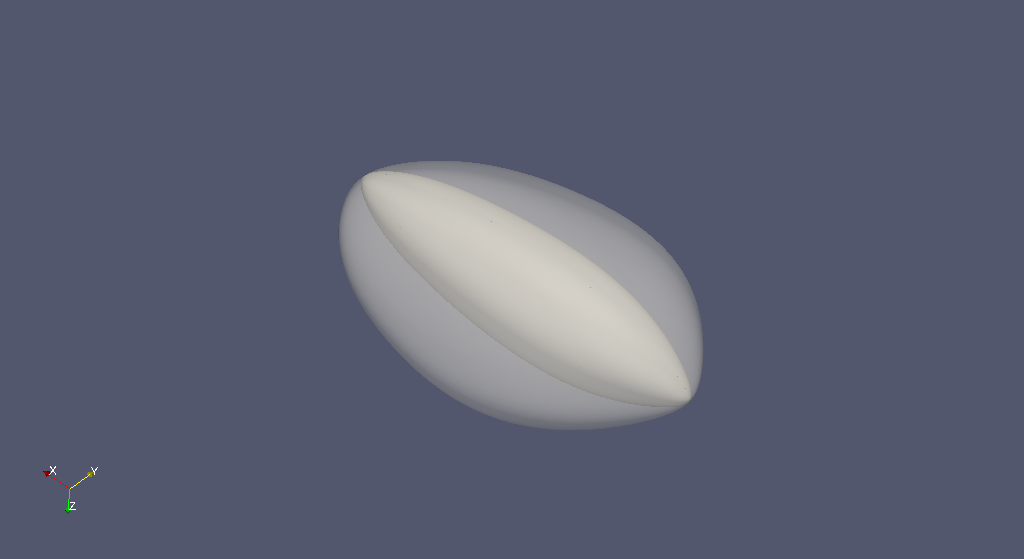
\includegraphics[width=200 pt]{rnd/effect_of_scaling.png}
	\caption{Effect of scaling }
	\label{Effect of scaling}
\end{figure}


\section{Methodology to generate geometry using \textit{Octave}}

Since the analysis work is being carried out using OpenFOAM\textsuperscript{\textregistered}, we need to input the geometry file to \textit{SnappyHexMesh} utility. OpenFOAM\textsuperscript{\textregistered} does not have any geometry creation utility. It has to be created using any commercial designing software and file has to be exported in \textbf{.stl} format. During optimization, calling the commercial CAD software every time to define simple mathematical shape is not a good practice. Instead we can define the geometry in Octave itself and carryout simulations. So, an existing MATLAB\textsuperscript{\textregistered} script by Bill [\citenum{BillMcDonald}] has been edited which takes the input of surface data  (X,Y and Z vectors) and writes them into .stl file. This .stl file can then be used in OpenFOAM\textsuperscript{\textregistered}. So, the need for commercial designing software has been eliminated.
\subsection{STL (file format)}
An ASCII STL file begins with the line
\begin{lstlisting}
solid name
\end{lstlisting}



where name is an optional string (though if name is omitted there must still be a space after solid). The file continues with any number of triangles, each represented as follows:
\begin{lstlisting}
facet normal ni nj nk 
	 outer loop	
		vertex v1x v1y v1z 
		vertex v2x v2y v2z 
		vertex v3x v3y v3z 
	 endloop 
endfacet 
\end{lstlisting}

where each n or v is a floating-point number in sign-mantissa-"e"-sign-exponent format, e.g., "2.648000e-002". The file concludes with the line,


\begin{lstlisting}
endsolid name
\end{lstlisting}

Thus the \textit{surf} data consisting of x,y,z coordinates of all the points are written into a text file in the above format and can be imported into OpenFOAM\textsuperscript{\textregistered} to carryout CFD simulation.

%%


%%% Local Variables: 
%%% mode: latex
%%% TeX-master: "../mainrep"
%%% End: 
